% Drawing 154/04-9 -- folder 154, batch 04, archive page 78 (PDF page 79).
% Transcription: figures dans la colonne de droite. En haut, au crayon : un arrangement de droites, dont un faisceau par un point, et une face $F$ orientée ($\omega_F$) ; sur son bord, les arêtes $a_\alpha$, $a_\beta$ et les sommets $\delta_0$, $\delta_1$, $\delta_2$, une flèche allant de $\delta_0$ à $\delta_1$. Au-dessous, en couleur : une droite vert clair $D = D_{\delta_0}$ orientée ($\omega_D$), des pseudo-droites vert clair en pointillé marquées $D_1$, $D_2$ au-dessus, et quatre paires de pseudo-droites rouges qui se croisent en des sommets dont $s_\alpha$, $s_\beta$ ; sur $D$, des segments épais noirs, l'un marqué $a'_\alpha$ ; une flèche courbe au point $x$ de $D$
% Kind: pencil arrangement with an oriented face; line D with pseudolines D_1, D_2 and four red crossings. Method 2 (schematic redraw from the facsimile). Status: partial.
% Notes: Right column. Top, in pencil: an arrangement of lines, one pencil of lines through a point, and an oriented face F (omega_F); on its boundary the edges a_alpha, a_beta and the vertices delta_0, delta_1, delta_2, an arrow from delta_0 to delta_1 (and one on to delta_2). Below, in colour: a light green line D = D_{delta_0} oriented (omega_D), light green dotted pseudolines D_1, D_2 above it, and four pairs of red pseudolines crossing at vertices among which s_alpha, s_beta; on D thick black segments, one marked a'_alpha; a curved arrow at the left end of D (the point x). Read from the page view; the red pairs and the pencil lines are approximate. Still differs from the facsimile: Read from the page view; the red pairs and the pencil lines are approximate.
% Coordinates: 1 unit = 1 mm = 1/100 of the crop width (bbox in page fractions: [0.61, 0.082, 0.959, 0.39]).
% Redrawn by Claude (claude-opus-5-5), issue #73, 2026-11-07; not checked by a human; not compiled (no TeX in the session).
% Revised by Claude (claude-opus-5-5) 2026-11-09 (issue #128) after Michel's check: vertices snapped to exact intersections (drawn points on their lines, meeting ends on the stroke they meet, near-concurrent lines through one computed point, curve ends on their rim); labels at \small as in folder 80 batch 3. Status: partial.
% Rights: reproduces part of the work -- behind RENDER_TRANSCRIPTS, never published by itself.
\documentclass[tikz,border=3pt]{standalone}
\usepackage{amsmath,amssymb}
\usetikzlibrary{patterns,arrows.meta}
\tikzset{Or/.style={orange!90!black}, Ye/.style={yellow!80!orange}, Lg/.style={green!60!black!70}, Dg/.style={green!45!black}, Br/.style={brown!80!black}, Rd/.style={red!85!black}, Bl/.style={blue!70!black}, Gy/.style={black!40}, pencil/.style={black!45}, struck/.style={black!35}, mark/.style={circle,draw,inner sep=1.3pt}, pt/.style={circle,fill,inner sep=0.9pt}, opt/.style={circle,draw,fill=white,inner sep=1.1pt}}
\begin{document}
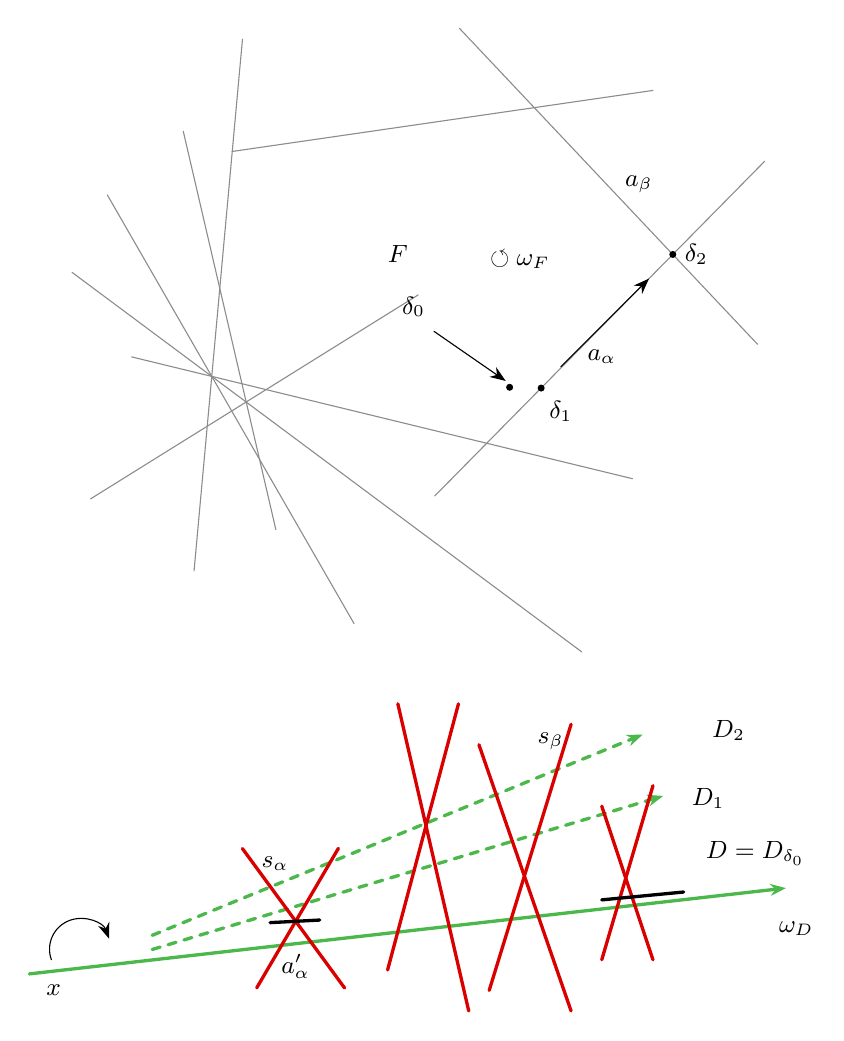
\begin{tikzpicture}[x=1mm,y=1mm,line cap=round,line join=round,font=\scriptsize]
\draw[pencil] (5.42,-32.2) -- (70.16,-80.41);
\draw[pencil] (9.91,-22.38) -- (41.24,-76.81);
\draw[pencil] (27.07,-2.58) -- (20.92,-70.11);
\draw[pencil] (19.55,-14.29) -- (31.31,-64.88);
\draw[pencil] (7.78,-60.97) -- (49.38,-35.07);
\draw[pencil] (25.77,-16.85) -- (79.2,-9.1);
\draw[pencil] (54.61,-1.2) -- (92.48,-41.34);
\draw[pencil] (51.49,-60.6) -- (93.39,-18.09);
\draw[pencil] (12.99,-42.94) -- (76.6,-58.41);
\node[inner sep=1pt] at (46.8,-29.9) {\small $F$};
\node[inner sep=1pt] at (62.3,-30.6) {\small $\circlearrowleft\omega_F$};
\node[inner sep=1pt] at (77.4,-21) {\small $a_\beta$};
\node[inner sep=1pt] at (72.7,-42.9) {\small $a_\alpha$};
\node[inner sep=1pt] at (48.8,-36.6) {\small $\delta_0$};
\node[inner sep=1pt] at (67.5,-49.9) {\small $\delta_1$};
\node[inner sep=1pt] at (84.7,-29.9) {\small $\delta_2$};
\node[pt] at (65,-46.9) {};
\node[pt] at (81.72,-29.93) {};
\node[pt] at (61,-46.8) {};
\draw[-{Stealth[length=2mm]}] (51.4,-39.7) -- (60.5,-46);
\draw[-{Stealth[length=2mm]}] (67.5,-44.2) -- (78.7,-33);
\draw[Lg,very thick,-{Stealth[length=2mm]}] (0,-121.3) -- (96.1,-110.4);
\node[inner sep=1pt] at (97.4,-115.6) {\small $\omega_D$};
\node[inner sep=1pt] at (92.2,-106) {\small $D=D_{\delta_0}$};
\draw[Lg,dashed,very thick,-{Stealth[length=2mm]}] (15.6,-118.2) -- (80.5,-98.7);
\node[inner sep=1pt] at (86.2,-99) {\small $D_1$};
\draw[Lg,dashed,very thick,-{Stealth[length=2mm]}] (15.6,-116.4) -- (77.9,-90.9);
\node[inner sep=1pt] at (88.8,-90.4) {\small $D_2$};
\draw[Rd,very thick] (27.06,-105.38) -- (40.04,-123.09);
\draw[Rd,very thick] (39.25,-105.35) -- (28.88,-123.07);
\draw[Rd,very thick] (46.8,-87) -- (55.8,-126);
\draw[Rd,very thick] (54.5,-87) -- (45.5,-120.8);
\draw[Rd,very thick] (57.1,-92.2) -- (68.8,-126);
\draw[Rd,very thick] (68.8,-89.6) -- (58.4,-123.4);
\draw[Rd,very thick] (72.7,-100) -- (79.2,-119.5);
\draw[Rd,very thick] (79.2,-97.4) -- (72.7,-119.5);
\draw[very thick] (30.58,-114.79) -- (36.88,-114.46);
\draw[very thick] (72.7,-111.9) -- (83.1,-110.9);
\node[inner sep=1pt] at (31.2,-107.3) {\small $s_\alpha$};
\node[inner sep=1pt] at (66.2,-91.7) {\small $s_\beta$};
\node[inner sep=1pt] at (33.8,-120.3) {\small $a'_\alpha$};
\draw[-{Stealth[length=2mm]}] (2.8,-119.5) arc[start angle=200, end angle=20, x radius=3.9, y radius=3.9];
\node[inner sep=1pt] at (3.1,-123.4) {\small $x$};
\end{tikzpicture}
\end{document}
